\chapter{An automatic state decomposition algorithm}
\label{chapter:automatic-state-decomposition}


%\section*{Gloss}

%The final piece of the puzzle in needed to begin to construct useful Markov models to study protein folding and dynamics was a way to choose the states for a given arbitrary macromolecule.
%It was clear that examination of potentials of mean force would not be a reliable means of defining these states in general, because for systems more complex than the alanine dipeptide, it was simply not clear what the complete set of slow degrees of freedom would be.
%Because of this, we set out to construct an algorithm capable of identifying approximations to metastable states from a set of equilibrium molecular dynamics trajectories.
%After digesting the theses of Willhelm Huisinga and Christof Sch\"{u}tte, then at the Zuse Institute of Berlin (referenced herein), I proposed an iterative algorithm for generating approximations to metastable states that would be suitable for proteins and other biomolecules.
%In the Summer of 2005, Nina Singhal (then a graduate student in Computer Science from the Pande lab at Stanford), Bill Swope (a computational chemist with the Blue Gene project at IBM Almaden), and I set out to implement, test, and refine this algorithm to the point where it was suitable for our purposes.
%The following research report, which will be submitted to the Journal of Chemical Physics, is the product of this work.

%\clearpage

\input chapters/automatic-state-decomposition/automatic-state-decomposition.tex

%% SUPP INFO %%%%%%%%%%%%%%%%%%%%%%%%%%%%%%%%%%%%%%%%%%%%%%%%%%%%%%%%%%%%%%%%%%%%

\begin{figure}[tb]
  \begin{center}
    \resizebox{\columnwidth}{!}{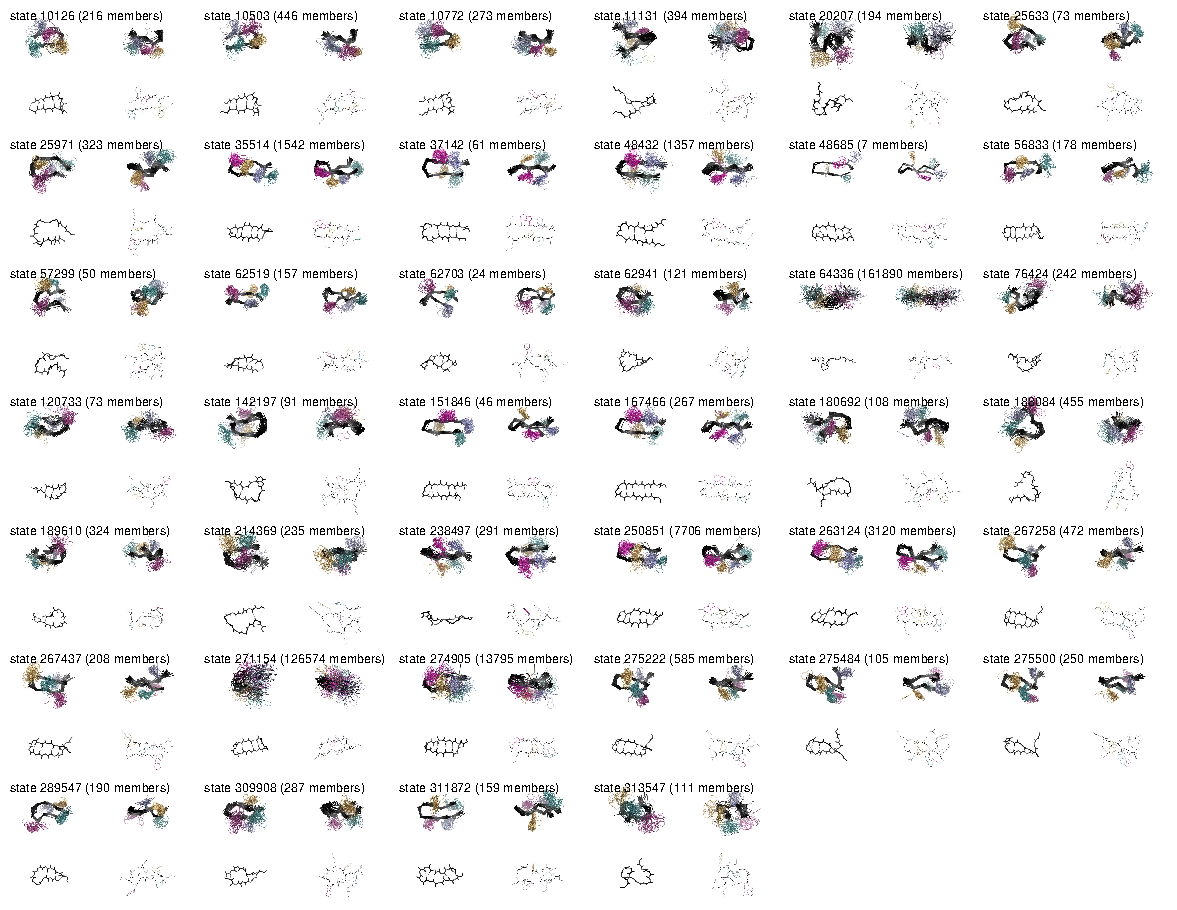
\includegraphics{chapters/automatic-state-decomposition/figures/trpzip2/trpzip2-states.pdf}}
  \end{center}
  \caption{{\bf Automatic state decomposition applied to trpzip2 to produce 40 macrostates.}}
  \label{automatic:figure:trpzip2-allstates}
\end{figure}
